\section{Method: the conformal notice alarm}\label{sec:method}

\begin{algorithm}
\caption{Conformal notice alarm (CNA) and its variants}\label{alg:cna}
\textbf{Input:} causal signal map; debounce $k$; lead time $\ell$; level $\alpha$; calibration units disjoint from those used to fit the signal.\\[2pt]
\textbf{Calibrate.} For each calibration unit $i$: compute its debounced running minimum $\rho^{(i)}$ and its critical level $V_i=\rho^{(i)}_{j_\ell}$ (Lemma~\ref{lem:crit}). If the unit was replaced or last seen alive at cycle $c_i$, use $U_i(c_i)$ instead (Lemma~\ref{lem:cens}). Set $\hat H=V_{(\lceil(n+1)(1-\alpha)\rceil)}$.\\[2pt]
\textbf{Operate.} Raise the alarm at the first row at which the signal has been at or below $\hat H$ for $k$ consecutive rows; schedule the replacement $\ell$ cycles later.\\[2pt]
\textbf{CNA-DA.} Given a cost ratio $\rho$ and a ceiling $\alpha_{\max}$, use $V_{(\hat q)}$ with
$\hat q=\arg\min_{q\ge q_0}\bigl[1+(\rho-1)\tfrac{n+1-q}{n+1}\bigr]\big/\overline{\text{use}}\bigl(V_{(q)}\bigr)$,
$q_0=\lceil(n+1)(1-\alpha_{\max})\rceil$, with the mean cycles of use estimated on the calibration units.\\[2pt]
\textbf{CNA+.} Replace the split by $K$-fold cross-fitting and raise the alarm by rule~\eqref{eq:cvplus}.\\[2pt]
\textbf{Online (new population).} Start from $\hat H$ of the old population; after each group of new units, update the level by~\eqref{eq:online} with the observed outcomes (Theorem~\ref{thm:online}).
\end{algorithm}

Calibration costs one pass over the calibration series (Fig.~\ref{fig:method}). The numerator of the CNA-DA objective replaces the empirical failure rate by its conformal value, which is never zero: with $q=n$ it is $1/(n+1)$. This is the difference from plain empirical cost minimisation, which sees no failure among calibration units at the edge of the feasible region and was fragile in the earlier study~\cite{prior}. By Corollary~\ref{cor:da} the failure probability of CNA-DA is at most $\alpha_{\max}$ whatever $\rho$ is.

\begin{figure*}[t]\centering
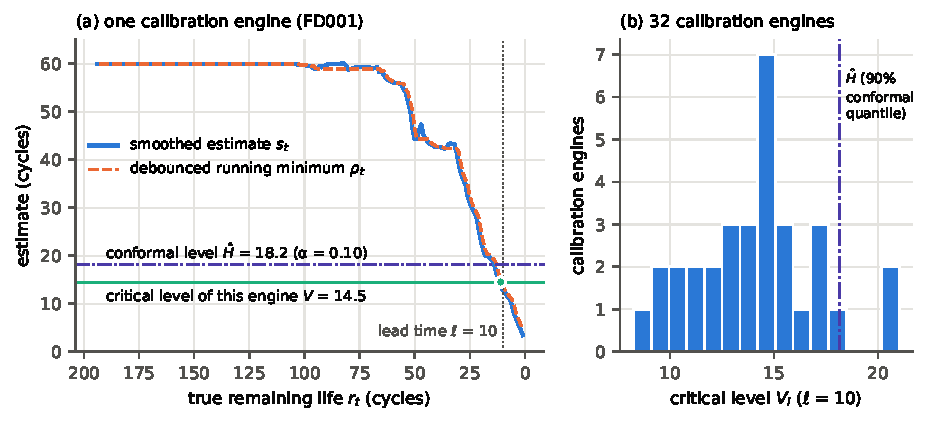
\includegraphics[width=0.92\textwidth]{figures/Fig1_method.pdf}
\caption{The conformal notice alarm on FD001 (fold~1, lead time 10 cycles). (a) The smoothed estimate of one calibration engine and its debounced running minimum $\rho_t$; the critical level $V$ is the value of $\rho$ at the last cycle with more than $\ell$ cycles left (dot). (b) Critical levels of the 32 calibration engines and the conformal level $\hat H$ at $\alpha=0.10$.}\label{fig:method}
\end{figure*}

\section{Experimental design}\label{sec:design}

The protocol (hypotheses H1--H5, datasets, policies, metrics and decision rules) was written and hashed with SHA-256 before the main experiments. Four amendments were hashed before their own experiments, each after the earlier results were known: H6--H8 (censoring, cross-fitting and the setting of Kamariotis et al.), H9 (comparators with the same information as the cross-fitted alarm), H10 (online calibration under batch shift) and H11--H13 (other learners and alarm settings). The hashes are not registry preregistrations; they show that the files have not changed since, and their timing rests on the repository history. The code was smoke-tested on one fold before each hash. One analysis was added afterwards and is labelled exploratory: the check of Corollary~\ref{cor:pac} on fold-level failure counts.

\textbf{Data.} We use the 218 PHM08 training engines (the development dataset of the earlier study), the C-MAPSS FD001--FD004 training sets (100, 260, 100 and 249 engines)~\cite{saxena2008}, N-CMAPSS reduced to one row per flight (99 engines in nine subsets, six temperature and speed channels)~\cite{ariaschao2021}, and 123 lithium-ion cells of Severson et al.~\cite{severson2019} in three batches (36, 43 and 44 cells; end of life at 80\,\% of nominal capacity), aggregated into blocks of 3 cycles fixed a priori. The engine datasets are simulations from one simulator family; the battery data are laboratory measurements. The 17 PRONOSTIA bearings~\cite{nectoux2012} of the earlier study are excluded: with at most about six calibration bearings per split, $\alpha\le0.10$ is not attainable.

\textbf{Splits and information.} Outer splits are five-fold cross-validation by unit (seed 2026), in which test units are exchangeable with training units, and, for transfer, leave-one-batch-out on the battery cells and leave-one-subset-out on N-CMAPSS. Inside each outer training set, 60\,\% of the units (proper training) fit the normalisation and the regressors and 40\,\% (calibration) are used for every selection, tuning and calibration step of every policy; CNA+ instead cross-fits all training units. Outer test units are scored once. The proper-training/calibration split is repeated three times (repetition~0 is primary). Disjointness of the unit sets is asserted in the code; features at row $t$ use rows $\le t$ only (tested by truncation); no test life enters any setting.

\textbf{Policies.} The signal is the regressor of the earlier study: histogram gradient boosting with absolute-error loss (500 iterations, learning rate 0.05, 31 leaves, at least 40 samples per leaf) on causal features of regime-normalised sensors (early-life baseline, exponentially weighted means, local slopes, age), target $\min(r,c)$~\cite{pedregosa2011}. Table~\ref{tab:policies} lists the policies. CNA uses settings fixed a priori (cap 60 cycles, battery 180; span 3; debounce 2), so that no selection touches the calibration units before the conformal step. Costs use lead times $\ell\in\{0,5,10,15\}$ cycles (battery $\{0,15,30,45\}$) and cost ratios $\rho\in\{5,10,20,50\}$; the primary lead time is 10 cycles (battery 30). The cost ratios are illustrative.

\begin{table*}[t]\footnotesize\setlength{\tabcolsep}{4pt}
\caption{Policies compared. All settings of learned policies are selected on calibration units; regressors are fitted on proper-training units (CNA+: cross-fitted on all training units).}\label{tab:policies}
\begin{tabular}{@{}p{0.2\textwidth}p{0.3\textwidth}p{0.3\textwidth}p{0.16\textwidth}@{}}
\toprule
Policy & Signal and trigger & Selected on calibration units & Guarantee \\
\midrule
CNA ($\alpha=0.05,0.10,0.20$) & GBM estimate (cap 60; battery 180 cycles), span 3, debounce 2, fixed a priori & $\hat H$ = conformal quantile of critical levels & $P(\text{fail})\le\alpha$ (Thm~\ref{thm:main}) \\
CNA-DA & As CNA & Order statistic minimising the cost bound, $\alpha_{\max}=0.10$ & $\le0.10$ (Cor.~\ref{cor:da}) \\
CNA+ / CNA+-DA & As CNA, five cross-fitted models & Count threshold of rule~\eqref{eq:cvplus} & $\le2\alpha+O(K/n)$ (Thm~\ref{thm:cvplus}) \\
Online CNA (new population) & As CNA & Level updated after each new unit by~\eqref{eq:online} from the old population's $\hat H$ & Long-run rate (Thm~\ref{thm:online}) \\
LB-all / LB-near & As CNA; alarm when $s_t-q_\alpha\le\ell+1$ & Conformal quantile of per-row residuals (all rows / rows with $r\le$ cap) & Per-row only \\
STW, window-tuned & GBM estimate (cap 40/60/90), span, debounce, shift & Most correct first warnings per $H$; $H$ by calibration cost & None \\
STW, cost-tuned (plain, 1-SE) & GBM estimate, span, debounce, threshold (2,160 settings) & Lowest calibration cost; 1-SE: largest notice within one bootstrap SE & None \\
Kamariotis P1 ($1/\rho$, optimised) & $P(r\le\ell+\Delta t\mid\text{estimate bin})$ from calibration rows (P-res) & Threshold $1/\rho$, or optimised on calibration cost & None \\
Age replacement & Age & Replacement age on training lives & None \\
Capacity trend (battery) & Discharge capacity extrapolated to 0.88\,Ah & As the STW and CNA counterparts, on all training cells & CNA version: Thm~\ref{thm:main} \\
CF versions (STW cost-tuned plain and 1-SE; P1 optimised and $1/\rho$) & Average of the five fold models of CNA+ & Out-of-fold predictions of all training units & None \\
\bottomrule
\end{tabular}
\end{table*}

\textbf{Metrics, tests and decision rules.} The primary metric is the \emph{failure-before-replacement rate} on test units, with Clopper--Pearson intervals~\cite{clopper1934} and a one-sided exact binomial test of rate $>\alpha$, Holm-adjusted over datasets~\cite{holm1979}. Notice at the alarm and wasted life measure what the guarantee costs. Cost rates are compared by paired bootstrap ratios over test units (2,000 resamples); a policy is called cheaper than another on a dataset if it is significantly cheaper in at least 8 of the 16 cost cells and significantly dearer in none. Window scores of estimate and constant are compared by the Tango score interval for paired proportions~\cite{tango1998} and two one-sided tests~\cite{schuirmann1987} with a margin of 5 points. Intervals cover the sampling of test units given fitted policies; the repetitions show the variability from the split.
